\documentclass[tikz,border=5pt]{standalone}
\usepackage[T1]{fontenc}
\usepackage{lmodern,amsmath,amssymb}
\usetikzlibrary{arrows.meta,calc,positioning,fit,backgrounds,shapes.geometric,matrix,decorations.pathreplacing,patterns}
\definecolor{ink}{gray}{0.08}
\definecolor{wash}{gray}{0.965}
\definecolor{soft}{gray}{0.45}
\tikzset{box/.style={draw=ink,line width=.65pt,fill=white,align=center,inner sep=4pt,outer sep=0pt,font=\small},flow/.style={draw=ink,line width=.65pt,-{Latex[length=1.8mm,width=1.3mm]},rounded corners=2pt},annotation/.style={font=\scriptsize,text=soft,align=center},groupbox/.style={draw=soft,dashed,line width=.45pt,fill=wash}}
\begin{document}
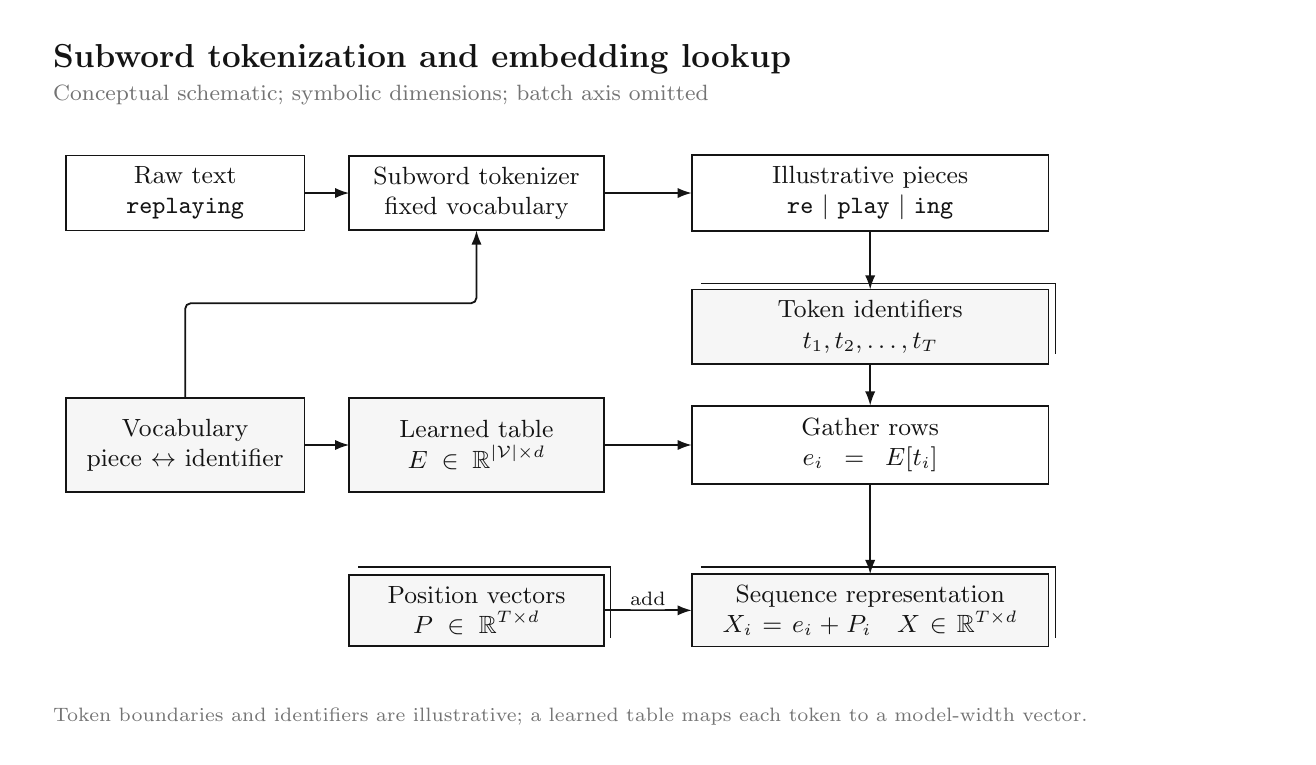
\begin{tikzpicture}[x=1cm,y=-1cm,font=\rmfamily,text=ink]

\path[use as bounding box] (0,0) rectangle (16,9);
\node[anchor=west,font=\large\bfseries] at (.2,.4) {Subword tokenization and embedding lookup};
\node[anchor=west,font=\footnotesize,text=soft] at (.2,.85) {Conceptual schematic; symbolic dimensions; batch axis omitted};
\begin{pgfonlayer}{background}
\end{pgfonlayer}
\node[box,minimum width=3cm,minimum height=0.9cm,text width=2.75cm] (text) at (2,2.1) {Raw text\\\texttt{replaying}};
\node[box,minimum width=3.2cm,minimum height=0.9cm,text width=2.95cm] (tok) at (5.7,2.1) {Subword tokenizer\\fixed vocabulary};
\node[box,minimum width=4.5cm,minimum height=0.9cm,text width=4.25cm] (pieces) at (10.7,2.1) {Illustrative pieces\\\texttt{re} $\mid$ \texttt{play} $\mid$ \texttt{ing}};
\node[box,fill=wash,minimum width=4.5cm,minimum height=0.9cm,text width=4.25cm] (ids) at (10.7,3.8) {Token identifiers\\$t_1,t_2,\ldots,t_T$};
\draw[ink,line width=.4pt] (8.549999999999999,3.2499999999999996) -- (13.049999999999999,3.2499999999999996) -- (13.049999999999999,4.15);
\node[box,fill=wash,minimum width=3cm,minimum height=1.2cm,text width=2.75cm] (vocab) at (2,5.3) {Vocabulary\\piece $\leftrightarrow$ identifier};
\node[box,fill=wash,minimum width=3.2cm,minimum height=1.2cm,text width=2.95cm] (table) at (5.7,5.3) {Learned table\\$E\in\mathbb{R}^{|\mathcal V|\times d}$};
\node[box,minimum width=4.5cm,minimum height=1.0cm,text width=4.25cm] (lookup) at (10.7,5.3) {Gather rows\\$e_i=E[t_i]$};
\node[box,fill=wash,minimum width=3.2cm,minimum height=0.9cm,text width=2.95cm] (pos) at (5.7,7.4) {Position vectors\\$P\in\mathbb{R}^{T\times d}$};
\draw[ink,line width=.4pt] (4.199999999999999,6.8500000000000005) -- (7.4,6.8500000000000005) -- (7.4,7.750000000000001);
\node[box,fill=wash,minimum width=4.5cm,minimum height=0.9cm,text width=4.25cm] (out) at (10.7,7.4) {Sequence representation\\$X_i=e_i+P_i\quad X\in\mathbb{R}^{T\times d}$};
\draw[ink,line width=.4pt] (8.549999999999999,6.8500000000000005) -- (13.049999999999999,6.8500000000000005) -- (13.049999999999999,7.750000000000001);
\begin{pgfonlayer}{background}
\draw[flow] (text.east) -- (tok.west);
\draw[flow] (tok.east) -- (pieces.west);
\draw[flow] (pieces.south) -- (ids.north);
\draw[flow] (ids.south) -- (lookup.north);
\draw[flow] (vocab.north) -- (2,3.5) -- (5.7,3.5) -- (tok.south);
\draw[flow] (vocab.east) -- (table.west);
\draw[flow] (table.east) -- (lookup.west);
\draw[flow] (lookup.south) -- (out.north);
\draw[flow] (pos.east) -- (out.west) node[midway,above,fill=white,inner sep=1.5pt,font=\scriptsize] {add};
\end{pgfonlayer}
\node[anchor=west,align=left,font=\scriptsize,text=soft,text width=15.6cm] at (.2,8.75) {Token boundaries and identifiers are illustrative; a learned table maps each token to a model-width vector.};
\end{tikzpicture}
\end{document}
